\documentclass[]{tufte-handout}

% ams
\usepackage{amssymb,amsmath}

% utf8 encoding
\usepackage[utf8]{inputenc}

% graphix
\usepackage{graphicx}
\setkeys{Gin}{width=\linewidth,totalheight=\textheight,keepaspectratio}

% booktabs
\usepackage{booktabs}

% url
\usepackage{url}

% hyperref
\usepackage{hyperref}

% units.
\usepackage{units}

% pandoc syntax highlighting

% longtable

% multiplecol
\usepackage{multicol}

% lipsum
\usepackage{lipsum}

% strikeout
\usepackage[normalem]{ulem}
 
% morefloats
\usepackage{morefloats}

% title / author / date
\title{Introducción al PLN \textbar{} ProgPLN}
\author{Víctor Peinado
\href{mailto:v.peinado@filol.ucm.es}{v.peinado@filol.ucm.es}}
\date{8-9 de octubre de 2015}


\begin{document}

\maketitle



\section{¿Qué es el PLN?}\label{que-es-el-pln}

El Procesamiento del Lenguaje Natural
(PLN)\footnote{En inglés, \textit{Natural Language Processing} (NLP) o mejor \#NLProc.}
es el estudio científico del lenguaje desde un punto de vista
computacional.

Es un área claramente multidisciplinar: lingüística, ingeniería,
inteligencia artificial, informática, psicología, etc.

El PLN se interesa en proporcionar modelos computacionales para
describir, modelar o reproducir distintos fenómenos lingüísticos.
Tradicionalmente, estos modelos han tenido dos aproximaciones
diferentes:

\begin{enumerate}
\def\labelenumi{\arabic{enumi}.}
\item
  sistemas basados en conocimiento: en problemas que podemos modelar,
  proporcionamos conocimiento lingüístico formalizado.
\item
  sistemas basados en estadística: en problemas que no podemos modelar,
  proporcionamos ingentes cantidades de datos (colecciones de
  documentos) y dejamos que la máquina cree el modelo a partir del
  cálculo de probabilidades y la detección de patrones de uso.
\end{enumerate}

\subsection{Tareas típicas del PLN}\label{tareas-tipicas-del-pln}

Una buena manera de conocer los temas que trata un área de investigación
es revisar el programa de los congresos más
importantes:\footnote{http://www.cs.rochester.edu/$\sim$tetreaul/conferences.html}

\begin{itemize}
\item
  ACL 2015: \emph{call for
  papers}\footnote{http://acl2015.org/call\_for\_papers.html} y
  programa\footnote{http://acl2015.org/program.html}
\item
  EMNLP 2015: \emph{call for
  papers}\footnote{http://www.emnlp2015.org/call.html} y
  programa\footnote{http://www.emnlp2015.org/program.html}
\item
  COLING 2014: \emph{call for
  papers}\footnote{http://www.coling-2014.org/call-for-papers.php} y
  programa\footnote{http://www.coling-2014.org/schedule.php}
\item
  SEPLN 2015: \emph{call for
  papers}\footnote{http://gplsi.dlsi.ua.es/sepln15/es/2-convocatoria-de-comunicaciones}
  y programa\footnote{http://gplsi.dlsi.ua.es/sepln15/es/node/52}
\end{itemize}

De este modo, podemos identificar algunas de las tareas más comunes del
área:

\begin{itemize}
\item
  Desambiguación semántica (\emph{word sense disambiguation}) y
  reconocimiento de entidades (\emph{named entities recognition}).
\item
  Análisis morfo-sintáctico
  (\emph{\href{http://nbviewer.ipython.org/gist/vitojph/5465948}{PoS
  tagging}/\href{http://nbviewer.ipython.org/gist/vitojph/5524353}{parsing}})
\item
  Traducción automática (\emph{machine translation}):
  \href{http://translate.google.es}{Google Translate}
\item
  Extracción de información (\emph{information extraction}):
  \href{https://www.tripit.com/}{TripIt}
\item
  Reconocimiento del habla (\emph{automatic speech reconition}) y
  síntesis de voz (\emph{speech synthesis}):
  \href{http://www.google.com/insidesearch/features/voicesearch/index-chrome.html}{Google
  Voice Search}
\item
  Recuperación de información (\emph{information retrieval}):
  \href{}{Google Search}, \href{http://www.bing.com}{Bing} y
  \href{http://www.wolframalpha.com/}{Wolfram\textbar{}Alpha}
\item
  Resumen automático (\emph{automatic summarization}) y generación
  automática de textos:
  \href{http://www.latimes.com/local/earthquakes/}{Quakebot} y
  \href{http://automatedinsights.com/}{Automated Insights}
\item
  Búsqueda de respuestas (\emph{question answering}):
  \href{http://www.ask.com}{Ask.com},
  \href{http://www.youtube.com/watch?v=WFR3lOm_xhE}{Watson}
\item
  Análisis de opiniones (\emph{sentiment analysis})
  \href{http://demos.bitext.com/naturalopinions/}{NaturalOpinions}
\item
  Comprensión del lenguaje natural (\emph{natural language
  understanding}): \href{http://www.apple.com/es/ios/siri/}{Siri},
  \href{https://support.google.com/websearch/answer/2940021?hl=es}{Ok
  Google} y
  \href{http://windows.microsoft.com/es-es/windows-10/getstarted-what-is-cortana}{Cortana}
\end{itemize}

\subsection{Problemas resueltos y cuestiones
abiertas}\label{problemas-resueltos-y-cuestiones-abiertas}

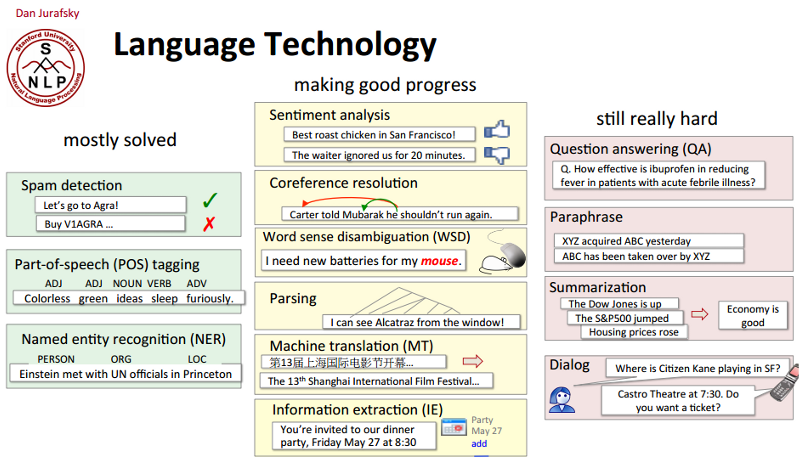
\includegraphics{img/langtech-progress.png}

\section{¿Por qué es tan difícil el
PLN?}\label{por-que-es-tan-dificil-el-pln}

El lenguaje natural es eminentemente \textbf{ambiguo}:. Esta es la
principal diferencia entre lenguas naturales y lenguajes artificiales.

Esta ambigüedad existe a varios niveles:

\begin{itemize}
\item
  ambigüedad fonética y fonológica: \emph{vaca/baca}, \emph{casa/caza},
  \emph{has sido tú/has ido tú}
\item
  ambigüedad morfológica: \emph{casa, beso, río, bajo}
\item
  ambigüedad sintáctica: \emph{Ayer me encontré a tu padre corriendo}
\item
  ambigüedad semántica: banco, pie,
\item
  ambigüedad de discurso: correferencia, resolución de anáforas
\end{itemize}

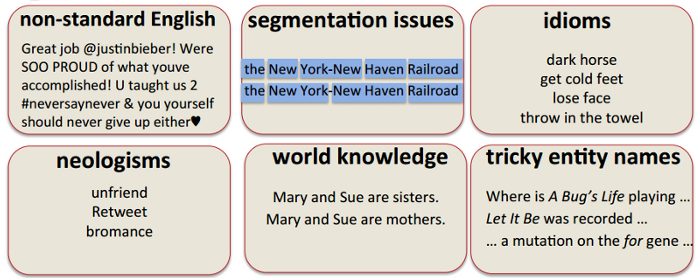
\includegraphics{img/nlp-difficulties.png}

Según la ACL (\emph{Association for Computational Linguistics}):
\emph{Computational Linguistics, or Natural Language Processing (NLP),
is not a new field}.\footnote{http://www.aclweb.org/aclwiki/index.php
?title=Frequently\_asked\_questions
\_about\_Computational\_Linguistics}, sin embargo no es sencillo definir
los límites de la disciplina. Así que podemos considerarla como un
conjunto de problemas relacionados con fenómenos lingüísticos y una
amalgama de soluciones computacionales, de distinto tipo dependiendo del
origen del investigador.

Según xkcd,\footnote{http://www.xkcd.org/114/} los lingüistas
computacionales han vivido muy bien hasta ahora vendiendo motos, así que
no se merecen más que nos metamos con ellos :-)
\footnote{http://www.explainxkcd.com/wiki/index.php/
114:\_Computational\_Linguists}

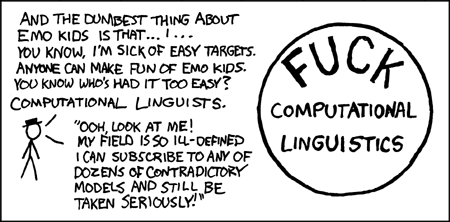
\includegraphics{img/xkcd_cl.png}


\end{document}
